\documentclass[fleqn]{article}[12pt]

\usepackage{amsmath}
\usepackage{amssymb}
\usepackage{pgfplots}
\usepackage[margin=1in]{geometry}
\usepackage{fancyhdr}
\usepackage{lastpage}
\usepackage{siunitx}
\usepackage{amsthm}
\usepackage{booktabs}


\setlength\parindent{0pt}

\cfoot{\thepage \hspace{1pt} / \pageref{LastPage}}
\newcommand{\integral}[4]{\int_#1^#2 \! #3 \, \mathrm{d}#4}
\newcommand{\dif}{\mathrm{d}}
\newcommand{\diracraw}{\left(\int_{-\infty}^{\infty} e^{i2\pi (f - \bar f)}\, dt\right)}
\usepackage{caption}
\captionsetup{justification=raggedright,singlelinecheck=false}
\DeclareMathOperator{\Imag}{Im}


\DeclareSIUnit\year{yr}
\DeclareSIUnit{\calorie}{cal}

\pgfplotsset{compat=1.14}

\newcommand{\M}{\mathbb{M}}
\newcommand{\W}{\mathbb{W}}
\newcommand{\R}{\mathbb{R}}


\begin{document}
    \begin{tabular}{l}
        ID \#33 \\
        Problem Set 9 \\
        Physics 202 \\
        \today
    \end{tabular}

\begin{enumerate}
    \item \begin{enumerate}
        \item Let $Z$ be the top of the air (or where pressure from above is negligible.) Then the pressure from above at point $z$ is
        \begin{equation*}
            P_{\text{above}} = \rho(Z-z)g
        \end{equation*}
        and the pressure below is
        \begin{equation*}
            P_{\text{below}} = \rho(Z+dz-z)g
        \end{equation*}
        Therefore,
        \begin{equation*}
            \frac{dP}{dz} = \frac{P_{\text{above}}-P_{\text{below}}}{dz} = -\rho g
        \end{equation*}

        \item Let $m$ be the average molar mass of the gas molecules. Density is defined as mass per volume, so, starting with $PV=nRT$,
        \begin{equation*}
            \rho = \frac{mn}{V} = \frac{P}{RT}
        \end{equation*}
        Then
        \begin{equation*}
            \frac{dP}{dz} = \rho g = -\frac{Pg}{RT} = -\frac{Pmg}{k_bT}
        \end{equation*}

        \item
        \begin{equation*}
            P(h) = P_0 + \int_{0}^{h} -\frac{Pmg}{k_bT}dz = P_0 \left.-\frac{g m z}{k_b T}\right|_{z=0}^{h} = P_0 - \frac{gmh}{k_b T}
        \end{equation*}

        \item Again using $PV=Nk_bT$,
        \begin{equation*}
            \rho(z) = \frac{N m}{V} = \frac{P(z)}{k_b T} = \frac{P_0 - \frac{gmz}{k_b T}}{k_b T} =
            \frac{P_0}{k_b T} - \frac{gmz}{(k_b T)^2}
        \end{equation*}

        \item The nitrogen-to-oxygen ratio increases with altitude because oxygen has a higher molar mass than nitrogen, so oxygen has a lower scale height and its partial pressure will decrease more quickly with altitude.
    \end{enumerate}

    \item When the bubbles are formed, they have the same temperature, which is the same as that of the lake. However, because the volumes increase as the bubbles rise, they both undergo an isobaric transition (in addition to an isochloric one.) Isobaric transitions involve work, and that energy comes from the thermal energy of the bubble. For the fast bubble, the temperature decrease counteracts the pressure decrease, since there is not enough energy to drive further expansion of the bubble.

    The slow bubble, however, maintains its temperature from the water, replenishing its thermal energy. Without the temperature drop to counteract the pressure drop, the slow bubble grows larger than the fast bubble.

    \item \begin{enumerate}
        \item Curve A is the isotherm, and curve B is the adiabat. The two can be distinguished because isotherms are symmetric along the $P=V$ line, since $P = c/V$, and $V = c/P$, for some constant $c$.

        \item Since the work is given by the integral of each curve between the start and endpoints, this depends on where the expansions take place. If they take place to the left of the $(V_i,P_i)$ point, the adiabatic expansion does more work. However, to the right of this point, the isothermal expansion does more work. The same holds for the contractions---to the left of the $(V_i,P_i)$ point, an adiabatic contraction requires more work, while on the right, an isothermal contraction requires more work.

        \item In an isothermal transition, $PV$ is always equal to some constant. In this case, that constant is $C = V_iP_i$, and the pressure as a function of volume is $P(V) = C/V = V_iP_i/V$. Then the total work done is
        \begin{equation*}
            Q = \int_{V_i}^{V_f} V_iP_i/V dV = P_iV_i(V_f/V_i) = P_iV_f
        \end{equation*}

        \item In an adiabatic process, $P_iV_i^\gamma = C$. Then the pressure as a function of volume is $P = C/V^\gamma$. Then the work done is
        \begin{equation*}
            Q = \int_{V_i}^{V_f} P_iV_i^\gamma/V^\gamma dV = \left.  \frac{P_iV_i^\gamma V^{1-\gamma}}{1-\gamma} \right|_{V=V_i}^{V_f} = \frac{P_iV_i^\gamma}{1-\gamma} (V_f^{1-\gamma}-V_i^{1-\gamma})
        \end{equation*}

        \item
        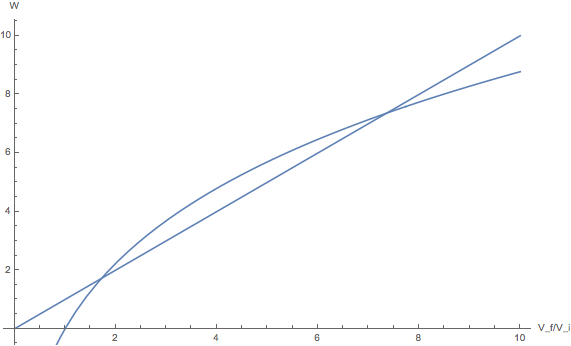
\includegraphics[width=0.8\textwidth]{graph3}
    \end{enumerate}
\end{enumerate}


\end{document}
